% Standalone RAKL provenance map (Paper VI): Papers I-V -> engine components.
% Build:  pdflatex papers_integration_map.tex  -> papers_integration_map.pdf
\documentclass[border=6pt]{standalone}
\usepackage{tikz}
\usepackage{amsmath}
\usepackage{helvet}\renewcommand{\familydefault}{\sfdefault}
\usetikzlibrary{positioning,arrows.meta,shapes.geometric,fit,backgrounds,calc}
\definecolor{oiblue}{HTML}{0072B2}
\definecolor{oiverm}{HTML}{D55E00}
\definecolor{oigreen}{HTML}{009E73}
\begin{document}
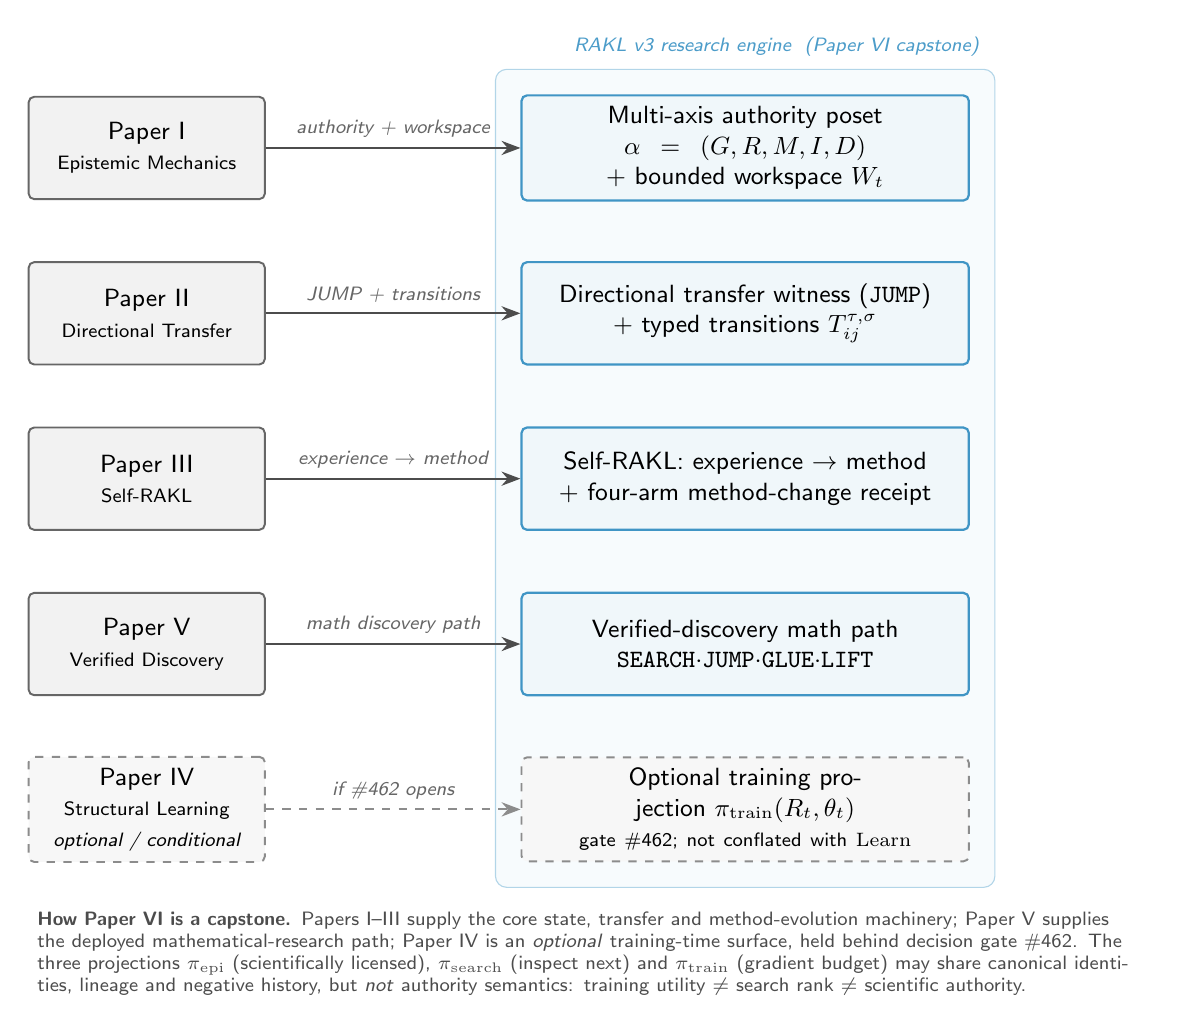
\begin{tikzpicture}[
  font=\small,
  >={Stealth[length=2.4mm]},
  paper/.style={rounded corners=2pt, draw=black!60, line width=0.7pt, align=center,
                inner sep=4pt, minimum height=13mm, minimum width=30mm, fill=black!5},
  comp/.style={rounded corners=2pt, draw=oiblue!75, line width=0.8pt, align=center,
               inner sep=4pt, minimum height=13mm, text width=54mm, fill=oiblue!6},
  opt/.style={rounded corners=2pt, draw=black!45, line width=0.7pt, align=center, dashed,
              inner sep=4pt, minimum height=13mm, text width=54mm, fill=black!3},
  prov/.style={->, line width=0.8pt, draw=black!70},
  lbl/.style={font=\scriptsize\itshape, text=black!60},
]
\def\ry{2.1}
% ---- left column: source papers I, II, III, V, IV ----
\node[paper] (p1) at (0, 0)      {Paper I\\{\scriptsize Epistemic Mechanics}};
\node[paper] (p2) at (0,-\ry)    {Paper II\\{\scriptsize Directional Transfer}};
\node[paper] (p3) at (0,-2*\ry)  {Paper III\\{\scriptsize Self-RAKL}};
\node[paper] (p5) at (0,-3*\ry)  {Paper V\\{\scriptsize Verified Discovery}};
\node[paper, draw=black!45, fill=black!3, dashed] (p4) at (0,-4*\ry)
      {Paper IV\\{\scriptsize Structural Learning}\\{\scriptsize\itshape optional / conditional}};

% ---- right column: engine components ----
\node[comp] (c1) at (7.6, 0)     {Multi-axis authority poset $\alpha=(G,R,M,I,D)$\\+ bounded workspace $W_t$};
\node[comp] (c2) at (7.6,-\ry)   {Directional transfer witness (\texttt{JUMP})\\+ typed transitions $T_{ij}^{\tau,\sigma}$};
\node[comp] (c3) at (7.6,-2*\ry) {Self-RAKL: experience $\to$ method\\+ four-arm method-change receipt};
\node[comp] (c5) at (7.6,-3*\ry) {Verified-discovery math path\\\texttt{SEARCH}$\cdot$\texttt{JUMP}$\cdot$\texttt{GLUE}$\cdot$\texttt{LIFT}};
\node[opt]  (c4) at (7.6,-4*\ry) {Optional training projection $\pi_{\mathrm{train}}(R_t,\theta_t)$\\{\scriptsize gate \#462; not conflated with $\operatorname{Learn}$}};

% ---- engine grouping panel ----
\begin{scope}[on background layer]
  \node[draw=oiblue!30, rounded corners=4pt, fill=oiblue!3,
        fit=(c1)(c4), inner sep=9pt] (engine) {};
\end{scope}
\node[lbl, text=oiblue!70, anchor=south east] at ([yshift=1pt]engine.north east)
      {RAKL v3 research engine \ (Paper VI capstone) \ };

% ---- provenance arrows ----
\draw[prov] (p1) -- node[lbl,above]{authority + workspace} (c1);
\draw[prov] (p2) -- node[lbl,above]{JUMP + transitions} (c2);
\draw[prov] (p3) -- node[lbl,above]{experience $\to$ method} (c3);
\draw[prov] (p5) -- node[lbl,above]{math discovery path} (c5);
\draw[prov, draw=black!45, dashed] (p4) -- node[lbl,above]{if \#462 opens} (c4);

% ---- projection footer: three views share identities, not authority ----
\node[anchor=north west, font=\scriptsize, text width=140mm, align=left, black!70]
      at ([yshift=-5mm]$(p4.south west)$)
      {\textbf{How Paper VI is a capstone.} Papers I--III supply the core state, transfer and method-evolution
       machinery; Paper V supplies the deployed mathematical-research path; Paper IV is an \emph{optional}
       training-time surface, held behind decision gate \#462. The three projections
       $\pi_{\mathrm{epi}}$ (scientifically licensed), $\pi_{\mathrm{search}}$ (inspect next) and
       $\pi_{\mathrm{train}}$ (gradient budget) may share canonical identities, lineage and negative history,
       but \emph{not} authority semantics: training utility $\neq$ search rank $\neq$ scientific authority.};
\end{tikzpicture}
\end{document}
